\documentclass[a4j]{jarticle}

\usepackage[dvipdfmx]{graphicx}
\usepackage{url}
\usepackage{here}
%\usepackage{listings}
\usepackage{amsmath,amssymb}
\usepackage[dvipdfmx]{color}

\setlength{\headsep}{-5mm}
\setlength{\oddsidemargin}{0mm}
\setlength{\textwidth}{165mm}
\setlength{\textheight}{230mm}
\setlength{\footskip}{20mm}

%% 本文
\begin{document}
\section{フロー図}

\begin{figure}[H]
\begin{center}
\resizebox{8cm}{!}{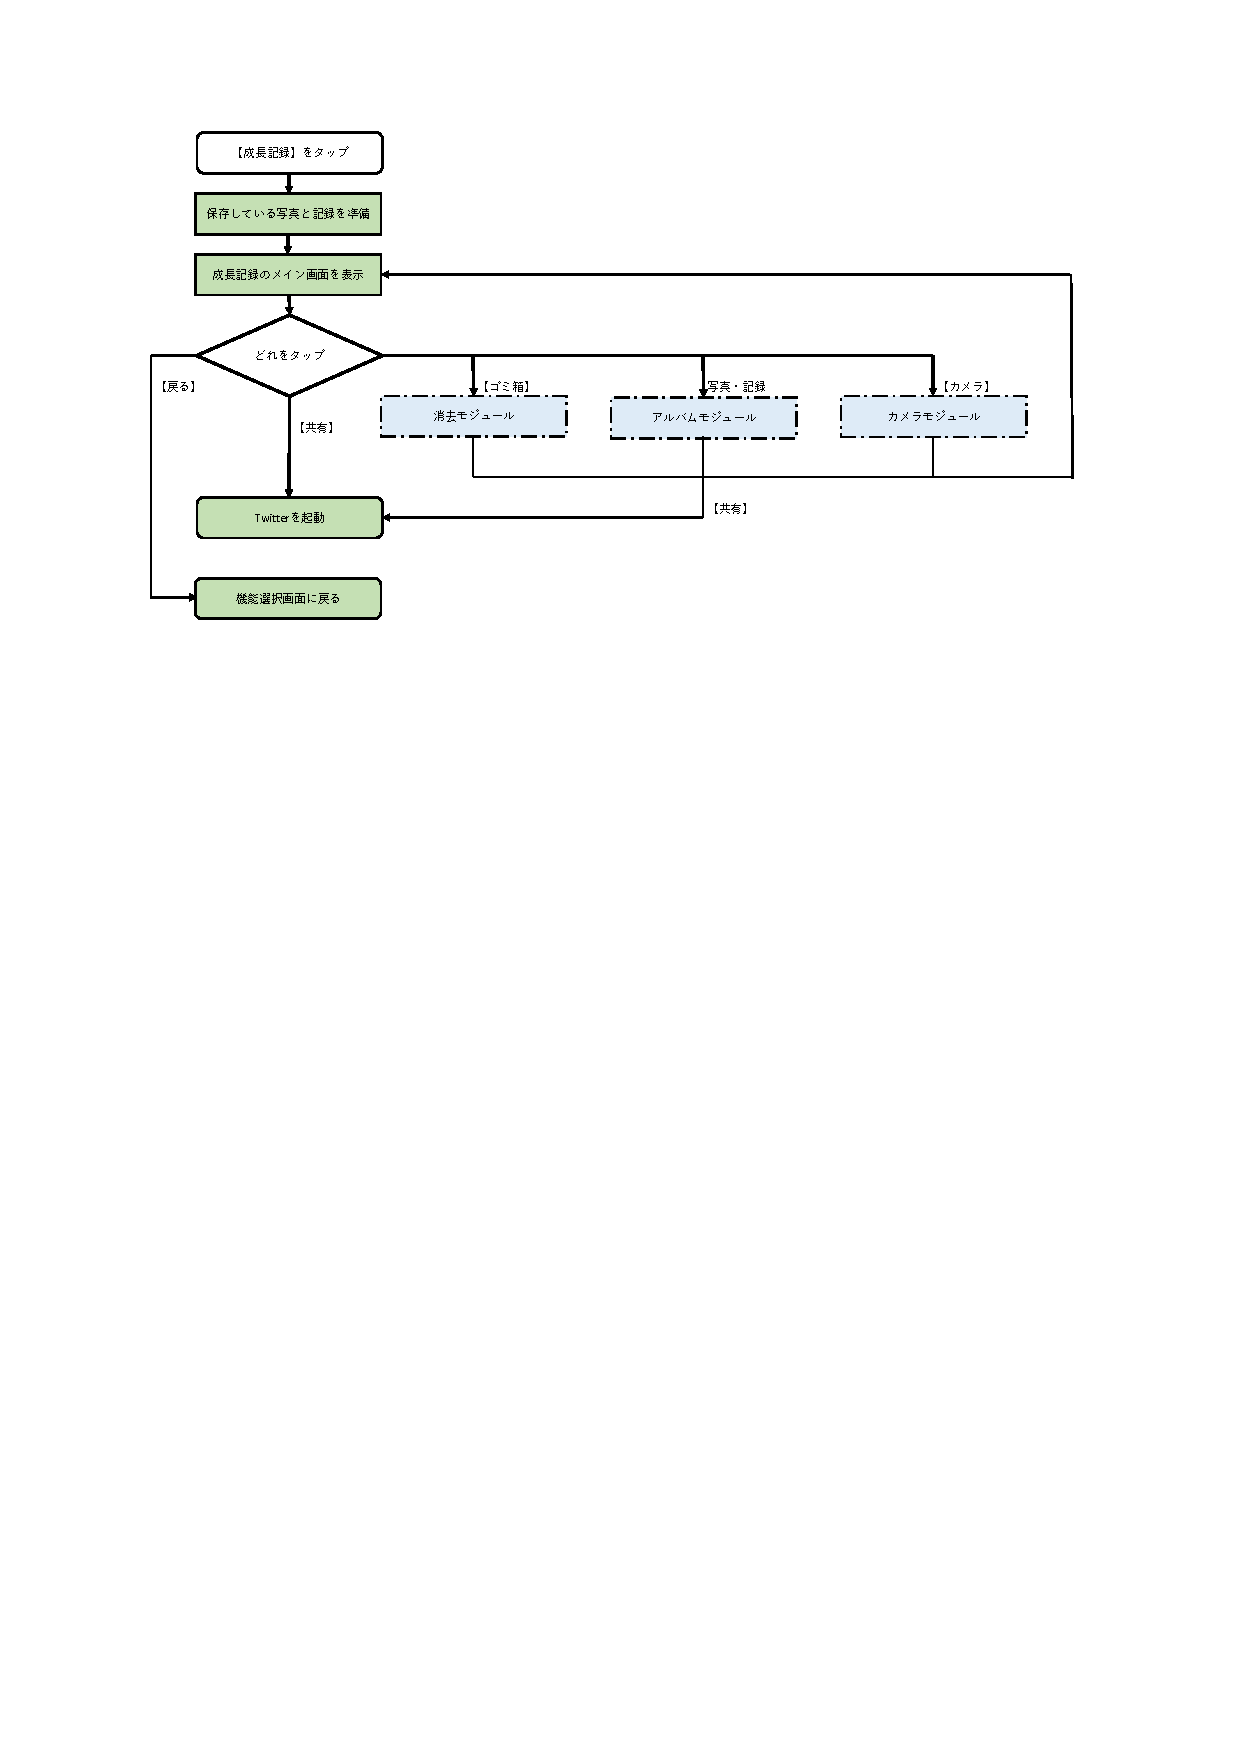
\includegraphics{成長記録全体.pdf}}
\caption{成長記録全体}
\label{allgrow}
\end{center}
\end{figure}

\begin{figure}[H]
\begin{center}
\resizebox{8cm}{!}{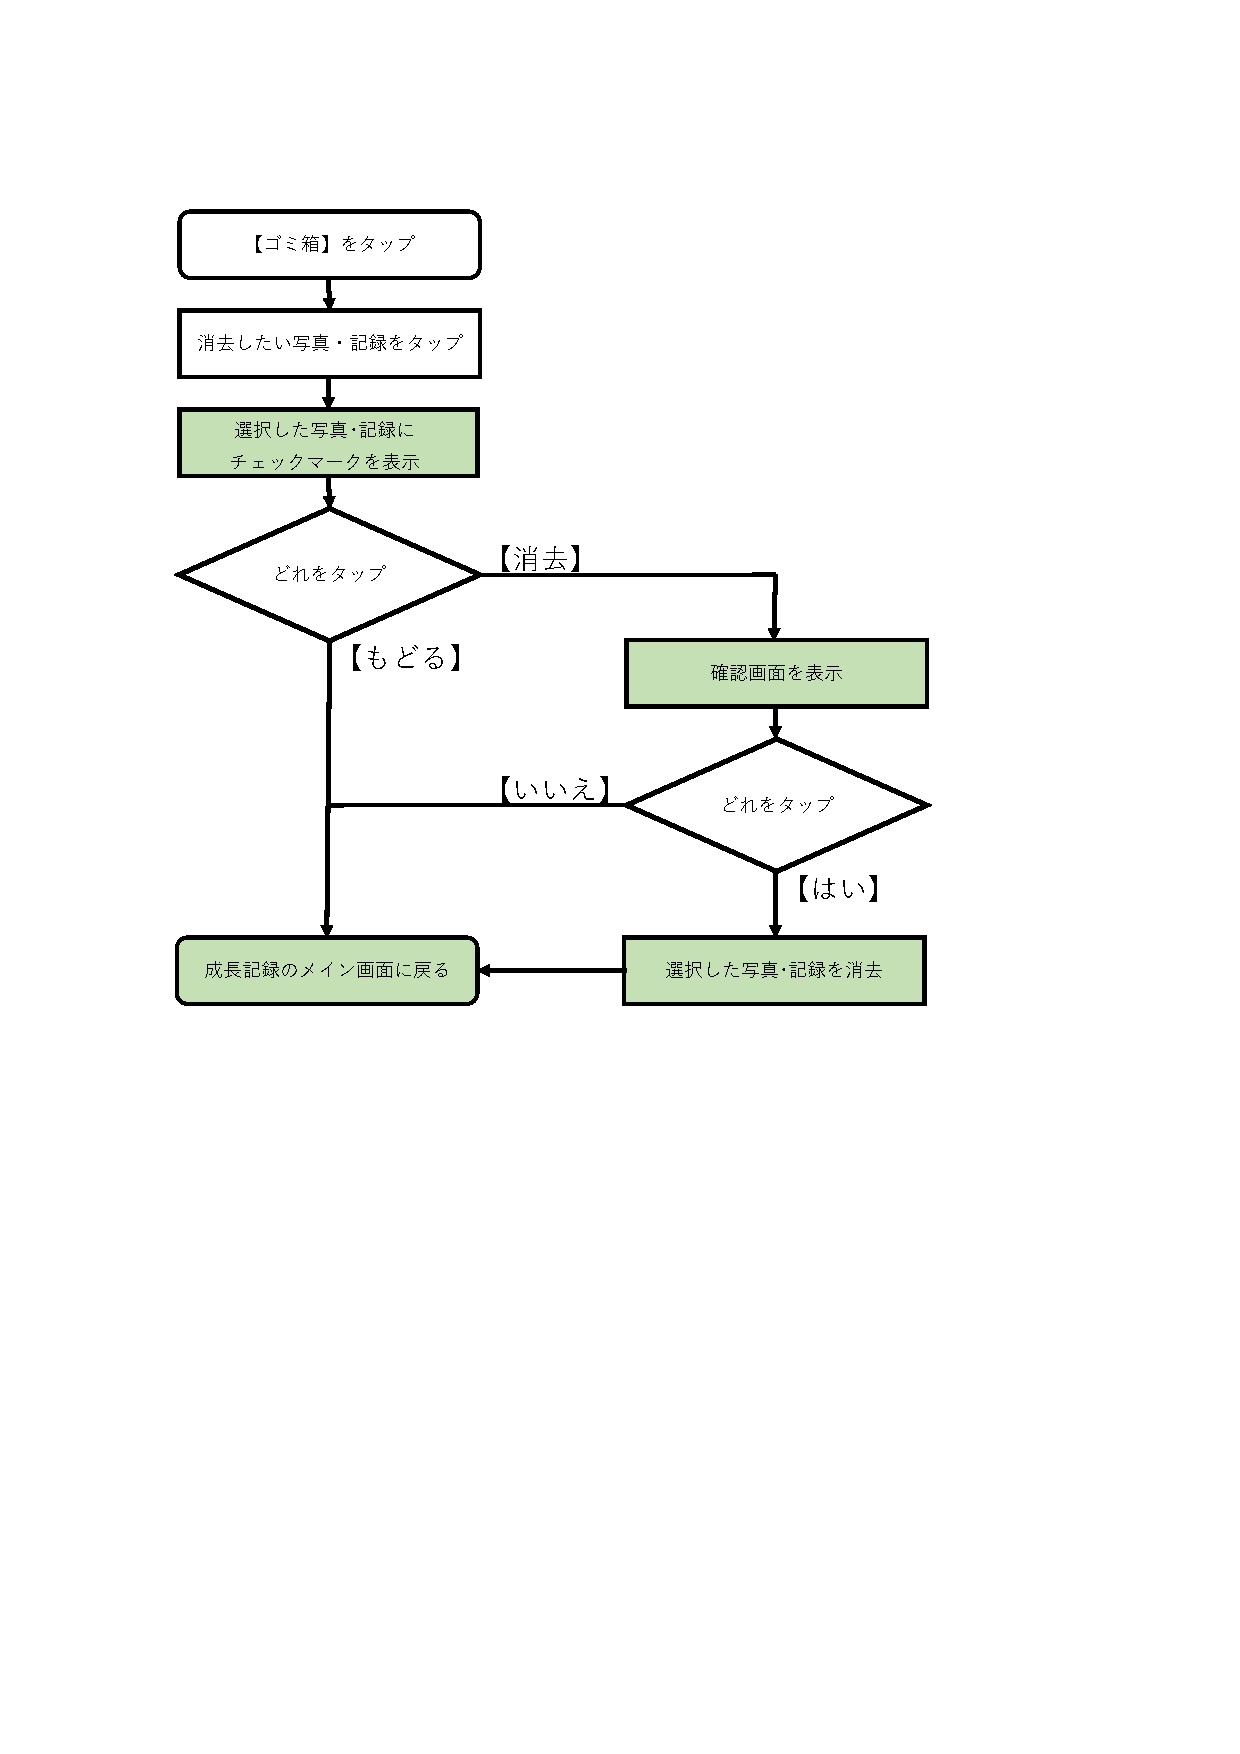
\includegraphics{消去モジュール.pdf}}
\caption{消去モジュール}
\label{deletemoju}
\end{center}
\end{figure}

\begin{figure}[H]
\begin{center}
\resizebox{8cm}{!}{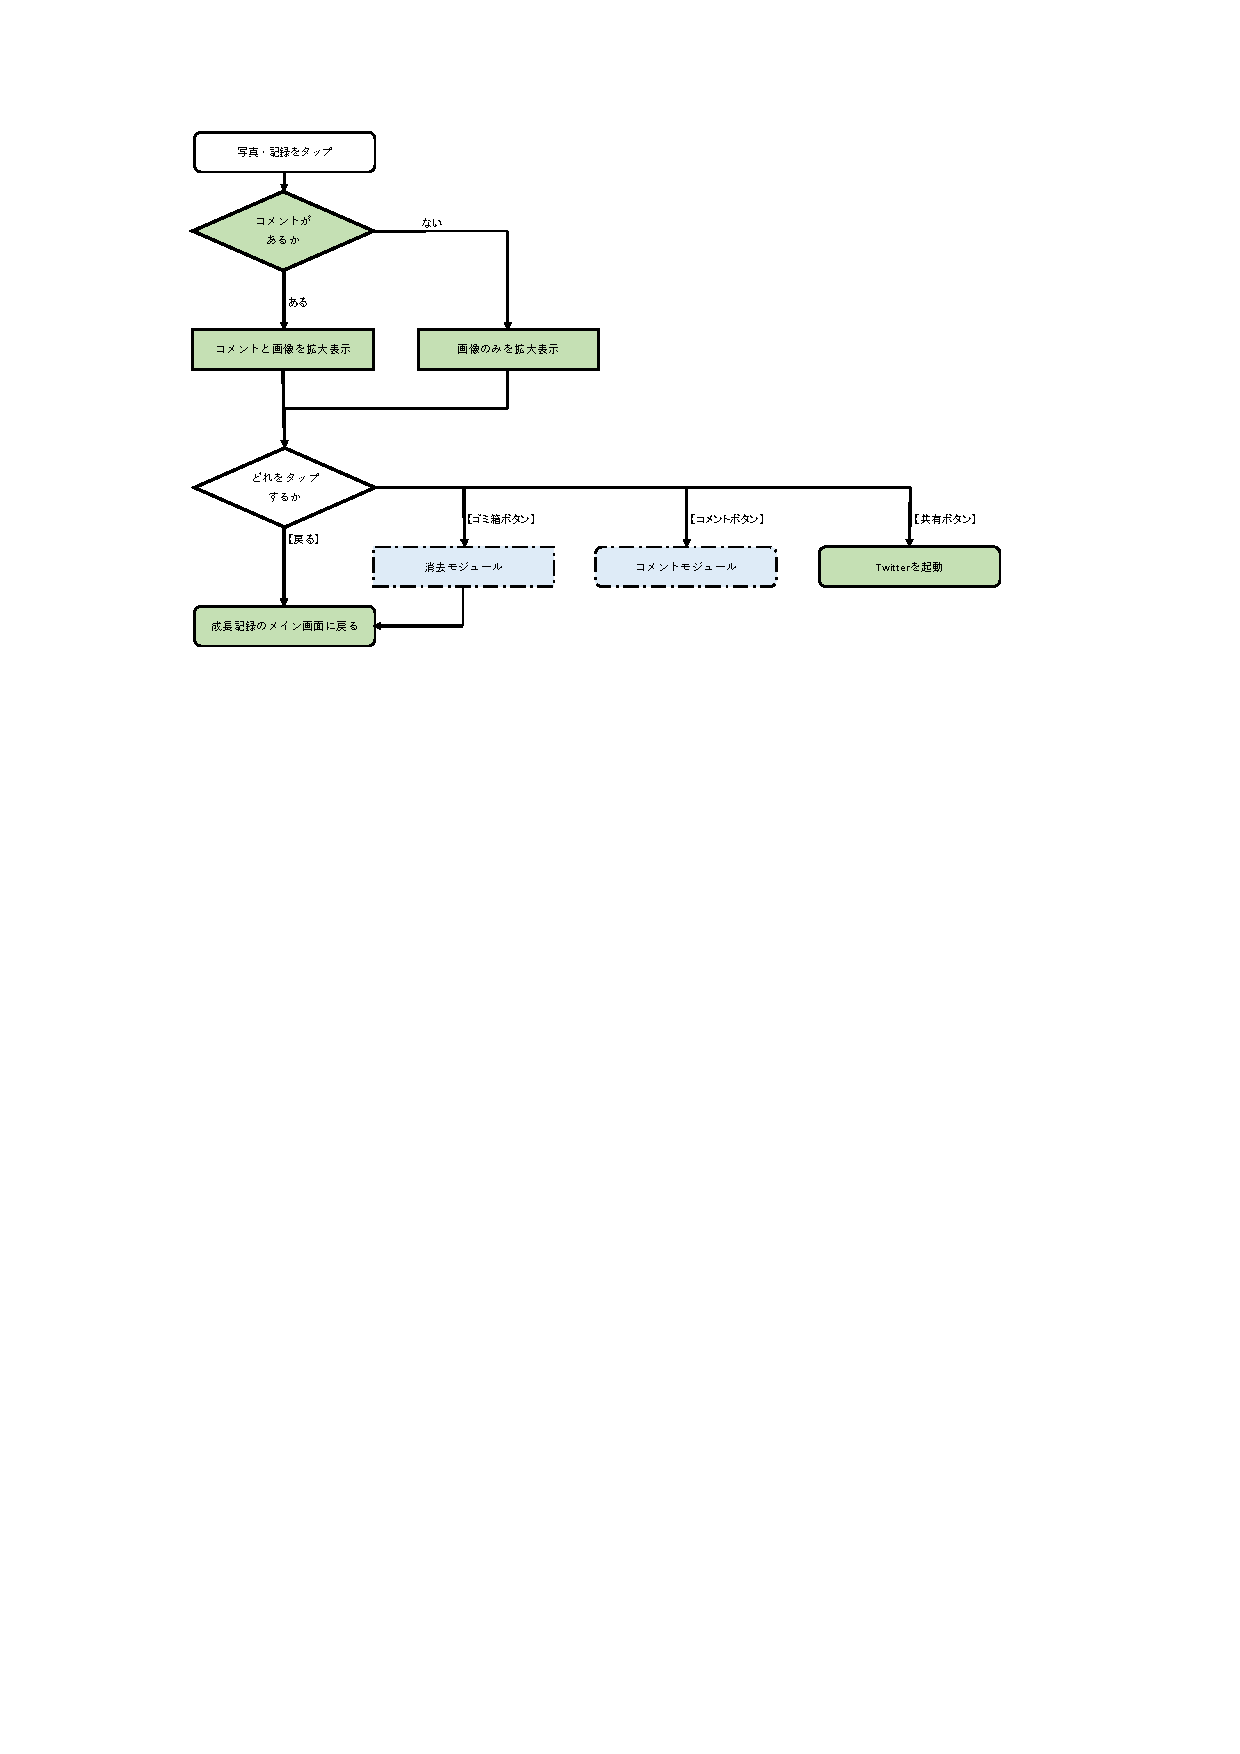
\includegraphics{アルバムモジュール.pdf}}
\caption{アルバムモジュール}
\label{alubammoju}
\end{center}
\end{figure}

\begin{figure}[H]
\begin{center}
\resizebox{8cm}{!}{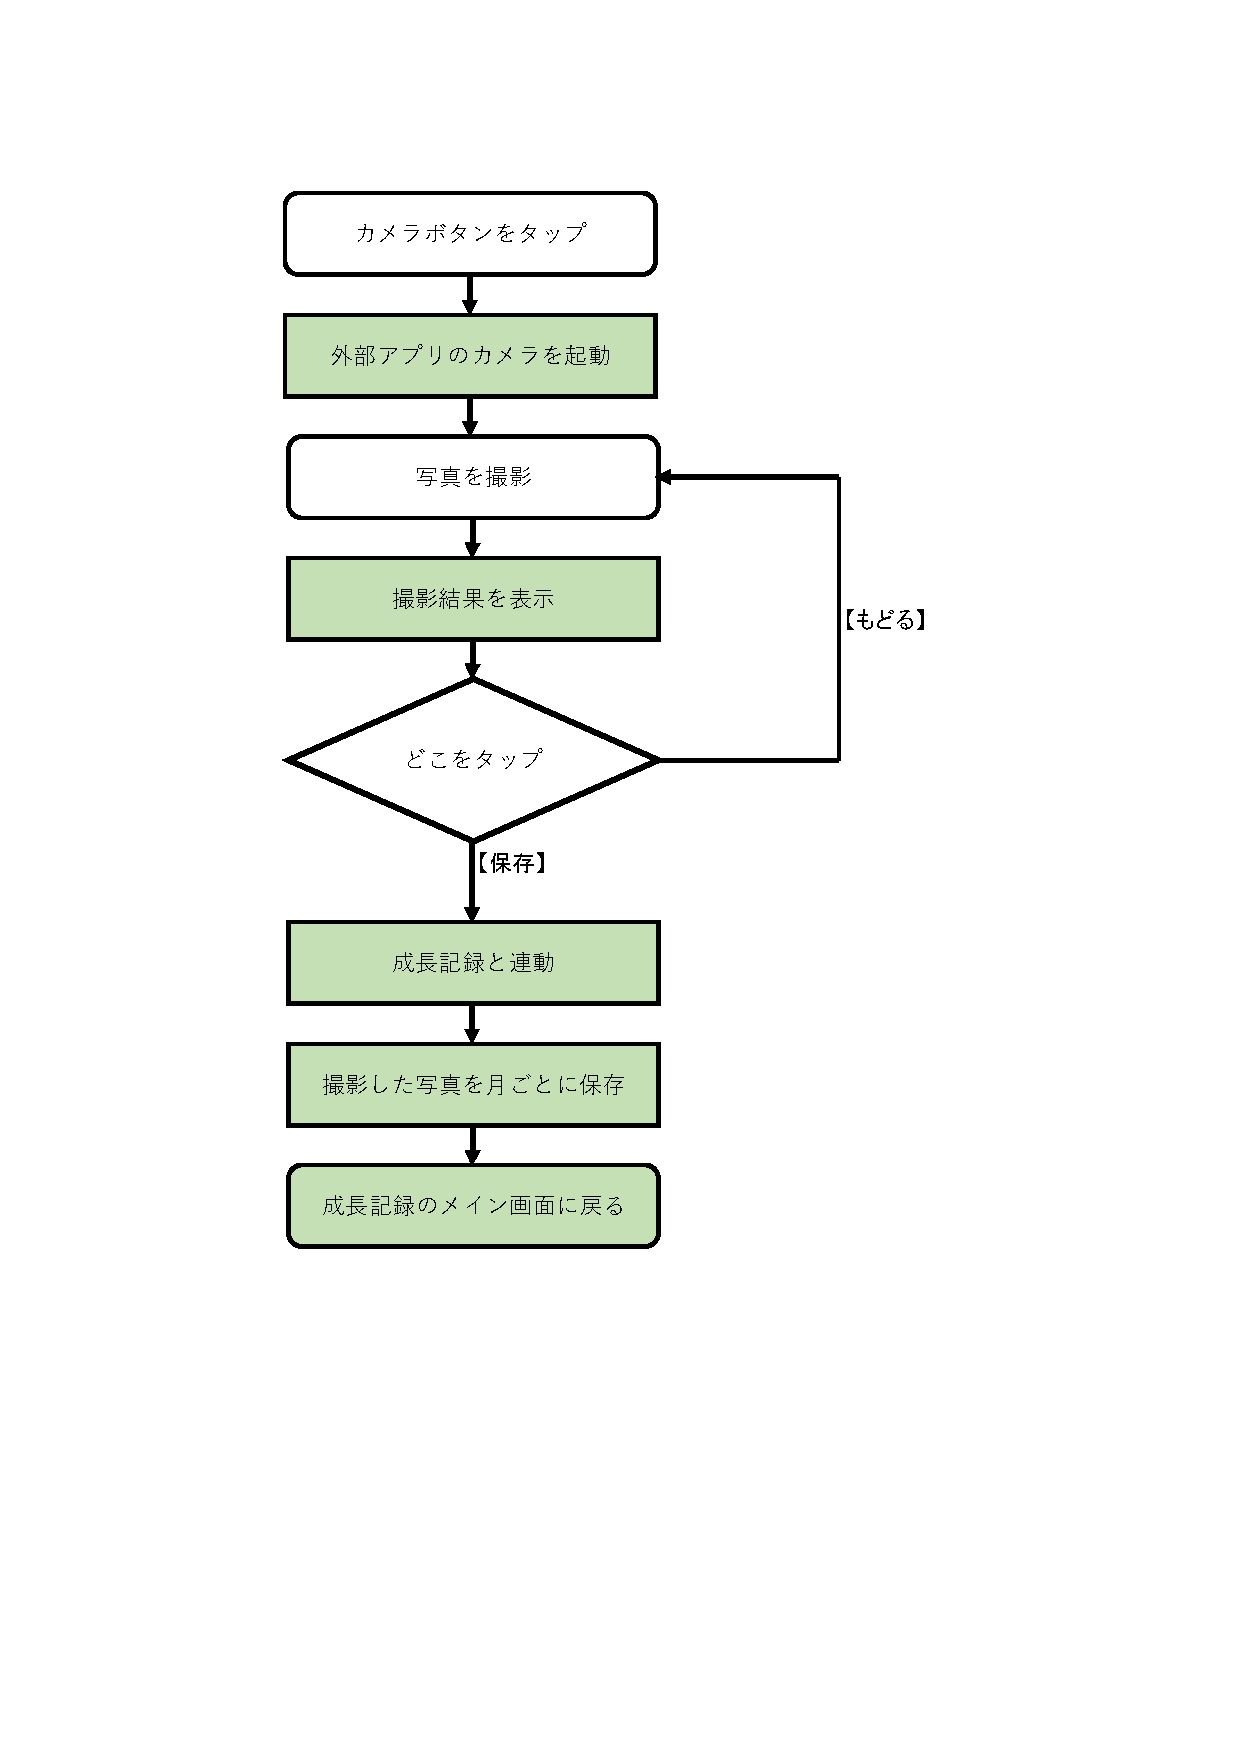
\includegraphics{カメラモジュール.pdf}}
\caption{カメラモジュール}
\label{cameramoju}
\end{center}
\end{figure}

\begin{figure}[H]
\begin{center}
\resizebox{8cm}{!}{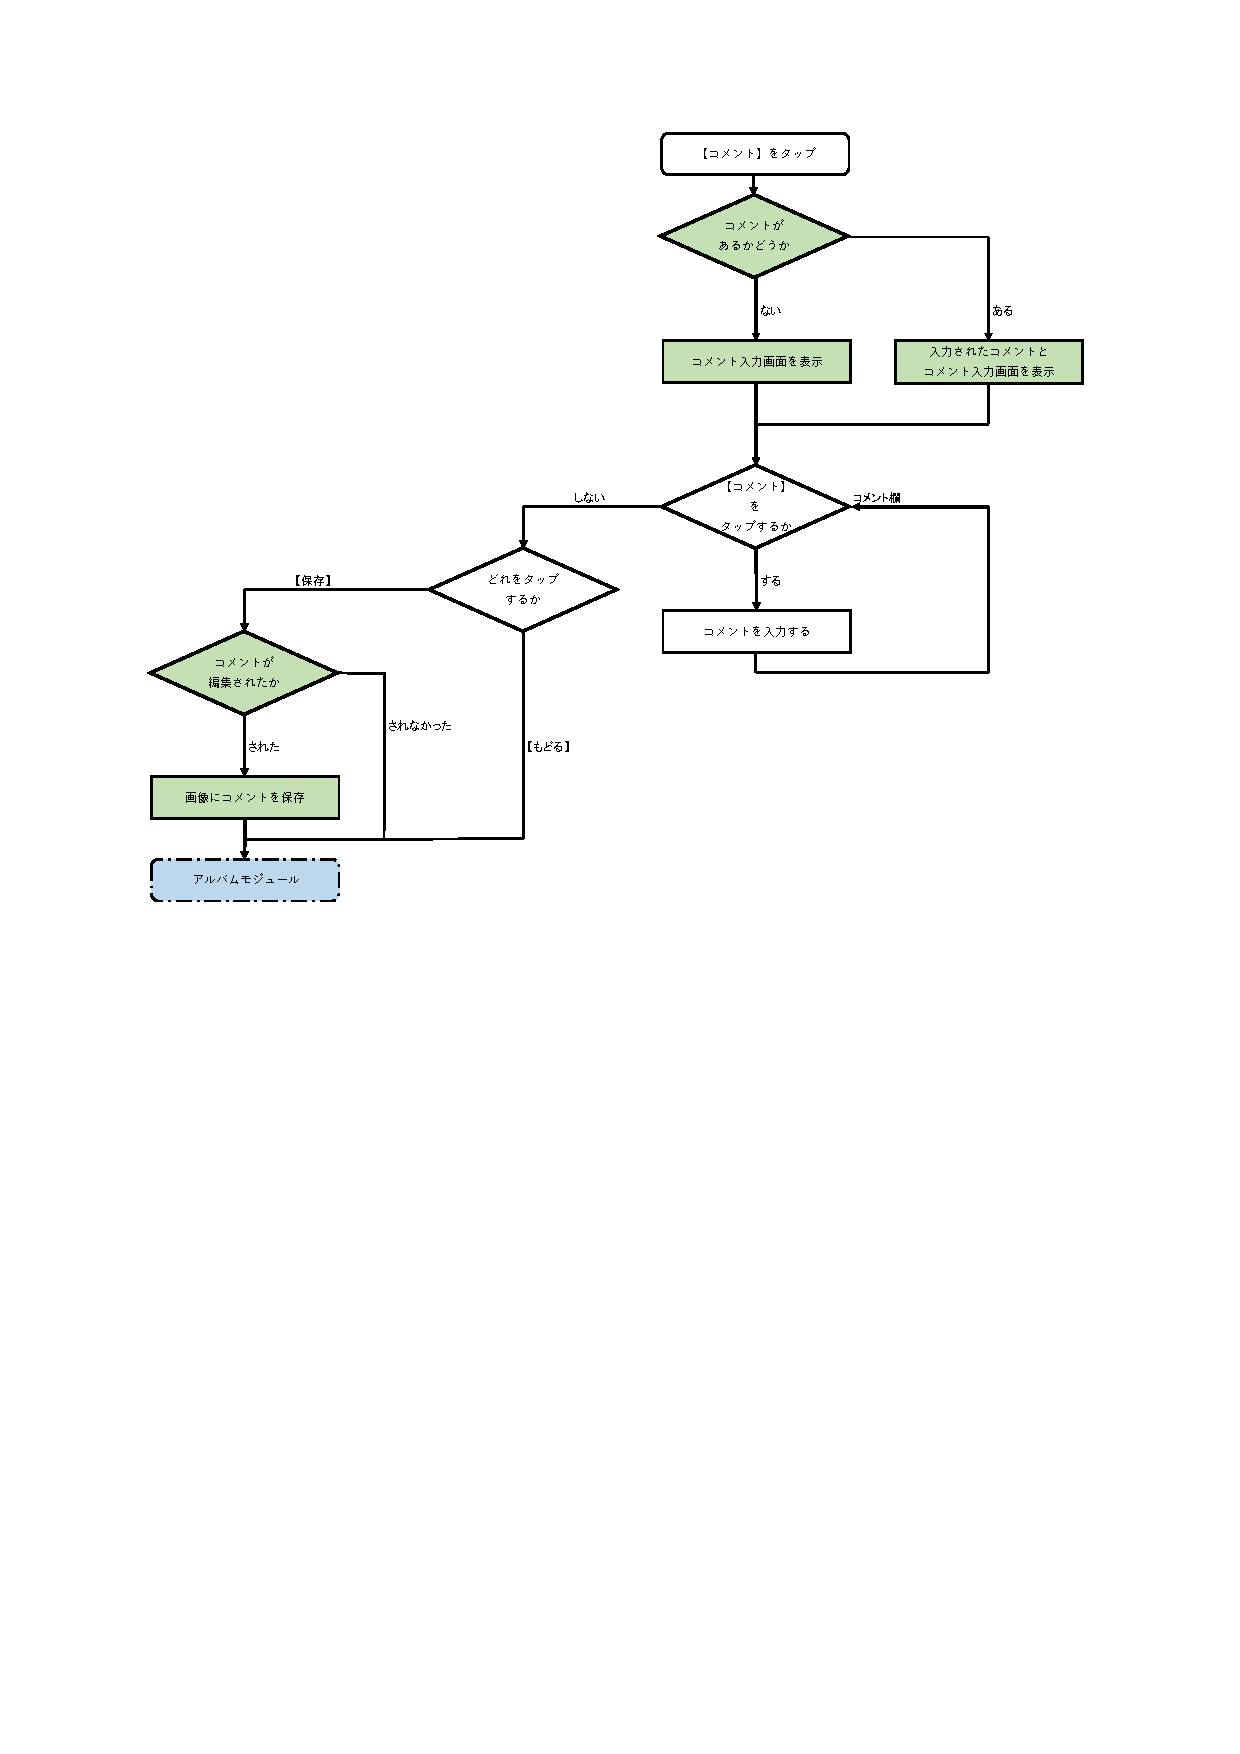
\includegraphics{コメントモジュール.pdf}}
\caption{コメントモジュール}
\label{comentmoju}
\end{center}
\end{figure}

\section{モジュール}
各モジュールの説明を行う

\subsection{成長記録全体}
〔概要〕利用者が保存した写真やゲームの記録などの閲覧や編集などを行うために使用する成長記録のメイン画面です。

機能としては、不要な写真や記録の削除、写真や記録の閲覧、写真の撮影、写真や記録をTwitterを介しての共有が行えます。

〔処理フロー〕
\begin{itemize}
\item 【ゴミ箱ボタン】をタップすることで消去モジュールを呼び出します。

\item 写真・記録を直接タップすることでアルバムモジュールを呼び出します。

\item 【カメラボタン】をタップすることでカメラモジュールを呼び出します。

\item 【共有ボタン】をタップすることで外部アプリであるTwitterを起動します。

\item 【もどるボタン】をタップすることで機能選択画面に戻ります。
\end{itemize}

\subsection{消去モジュール}
〔概要〕利用者が不要と判断した写真やゲームの記録の消去を行うために使用する機能です。

〔処理フロー〕
\begin{itemize}
\item 消去したい写真や記録をタップすることでその写真や記録にチェックマークが表示されます。その後、【消去】するか【もどるボタン】を選択します。
\item 【消去】を選んだ場合確認画面が表示されます。確認画面では【はい】と【いいえ】のボタンがあります。
\item 【はい】をタップすると選択した写真や記録が消去されます。
\item 【いいえ】をタップすると消去するか戻るかを選択する画面に戻ります。
\item 【もどるボタン】をタップした場合成長記録のメイン画面に戻ります。
\end{itemize}

\subsection{アルバムモジュール}
〔概要〕利用者が閲覧したい写真や記録をタップすることでそれを拡大表示して閲覧することができる機能です。

〔処理フロー〕
\begin{itemize}
\item 写真や記録タップした場合、それにコメントがついているかを判定します。コメントがあった場合はコメントを写真や記録と一緒に表示し、ない場合は写真や記録のみを拡大表示します。拡大表示した画面では【もどるボタン】,【ゴミ箱ボタン】,【コメントボタン】,【共有ボタン】が選択できます。
\item 【もどるボタン】をタップすることで成長記録のメイン画面に戻ることができます。
\item 【ゴミ箱ボタン】をタップすることで消去モジュールを呼び出します。
\item 【コメントボタン】をタップすることでコメントモジュールを呼び出します。
\item 【共有ボタン】をタップすることで外部アプリであるTwitterを起動します。
\end{itemize}

\subsection{カメラモジュール}
〔概要〕利用者が新しく写真を撮影したいときに使用する機能です。

〔処理フロー〕
\begin{itemize}
\item 外部アプリのカメラを起動し写真を撮影します。その後、【もどるボタン】か【保存ボタン】を選択します。
\item 【もどるボタン】をタップすることで写真を撮影する画面に戻ります。
\item 【保存ボタン】をタップすることで成長記録と連動します。その後、撮影した写真を月ごとに保存し成長記録のメイン画面に戻ります。
\end{itemize}

\subsection{コメントモジュール}
〔概要〕利用者が写真や記録にコメントを挿入したい、または既についているコメントを編集したい場合に使用する機能です。

〔処理フロー〕
\begin{itemize}
\item このモジュールに入ったときにその写真や記録にコメントが付与されているかを判定します。コメントがなければコメント入力画面のみ表示し、コメントがあればそのコメントとコメント入力画面を一緒に表示します。
\item コメント入力画面が表示されるとコメント欄をタップすることでコメントの書き込みが行えます。挿入、編集は何度でも行えます。
\item コメントの書き込みが終わった場合、もしくはコメントを書き込まなかった場合【保存ボタン】をタップするか、保存せずに【もどるボタン】をタップするかを選択します。
\item 【保存ボタン】をタップした場合コメントの内容が変更されたかを判定し、変更されていれば内容を保存してアルバムモジュールに戻ります。変更されていなければ保存せずにアルバムモジュールに戻ります。
\item 【もどるボタン】をタップすることで内容を保存せずアルバムモジュールに戻ります。
\end{itemize}

\end{document}
